\section{Resultados}

Conociendo los valores iniciales de la se\~nal limpia, el ruido proporcionado y
habiendo obtenido el resultado luego de aplicar los filtros, resulta muy
sencilla una primera aproximaci\'on a los resultados. La idea del experimento es
intentar que la se\~nal recuperada se parezca lo m\'as posible a la original
(sin ruido).

Fue muy simple, entonces, observar la diferencia entre la se\~nal recuperada y
la original de manera gr\'afica, ya sea a trav\'es de ploteos de se\~nales de 1
\'o 2 dimensiones como de la fuente misma como son las im\'agenes en 2
dimensiones.

Acompa\~nando esto por m\'etodos anal\'iticos como el PSNR (Relaci\'on Se\~nal a
Ruido de Pico) fue posible analizar que filtros resultan mejores que otros y en
que casos es mejor aplicar cada uno.

\subsection{Primeros resultados}

Experimentalmente pudimos observar que el filtro cero es bueno, pero el filtro 
exponencial y el promediador son bastante mejores en todos los casos. 
Para poder obtener un mejor filtrado del ruido, decidimos aplicar primero el 
filtro exponencial y luego el promediador, lo que result\'o en un filtrado muy 
bueno dando resultados muy parecidos a la se\~nal original. 

Los adjetivos utilizados se apoyan tanto en el campo sensorial (en las
im\'agenes y gr\'aficos) como en la medida deL PSNR. 

\subsection{Se\~nales en una dimensi\'on}

\subsubsection{Filtro Cero}

El primer filtro analizado fue el m\'as sencillo de implementar, el filtro cero.
Como mencionamos anteriormente, este filtro utiliza un umbral y env\'ia los
puntos que lo sobrepasan (tanto por arriba como por debajo) a cero.

\begin{figure}
\begin {center}
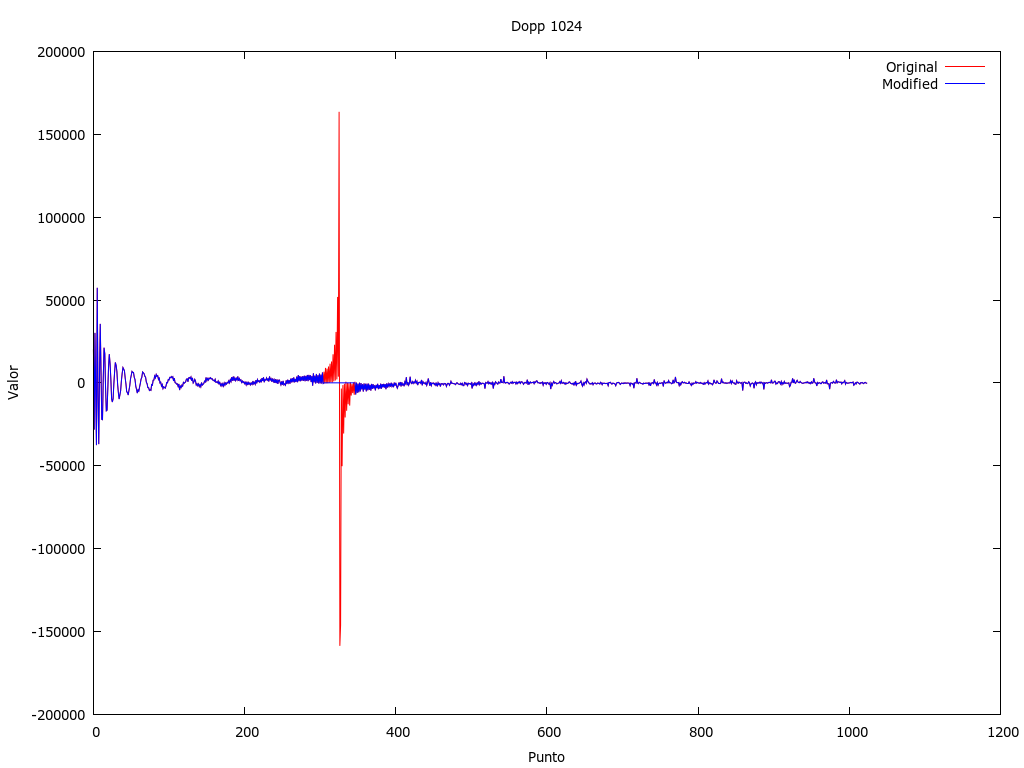
\includegraphics[width=360pt]{imagenes/dopp1024-sin100-zero-spec.png}
\end {center}
\caption{Se\~nal doppler provista por la c\'atedra, transformada, gr\'aficada
luego de aplicar ruido senoidal utilizando el multiplicador 100 (Rojo) y 
habiendo aplicado el filtro cero (azul)}
\label{fig:SinProm}
\end{figure}

Pudimos observar entonces que la se\~nal detecta frecuencias fuera del umbral y
las manda a cero. Este filtro carece de dos caracter\'isticas fundamentales
seg\'un demuestran los experimentos:

\begin{itemize}
	\item {\bf detecci\'on de ``zonas afectadas'':} Como el algoritmo no tiene en
cuenta el contexto a la hora de modificar un punto, la decisi\'on es mandar los
puntos duera del umbral al cero. Esto lleva a ``saltos'' pronunciados en la se\
~nal recuperada.

	\item {\bf elecci\'on de la correspondencia de los puntos fuera del umbral:}
El filtro decide enviar todos los elementos fuera del umbral al cero, con un
manejo de los m\'aximos y minimos globales (en el punto anterior se habla de
locales) se podr\'ia mejorar el resultado del filtro.
\end{itemize}

Sin embargo, como se aprecia en la im\'agen, los resultados son suficientemente
buenos teniendo en cuenta la simplicidad de la implementaci\'on del algoritmo.

\subsubsection{Filtro Exponencial}

Este filtro surge como una mejora del Filtro Cero. La idea que proviene de
observar los resultados provistos por el Filtro Cero est\'a relacionada con la
noci\'on de agregado de ``zona afectada'' ante la detecci\'on de un punto fuera
del umbral determinado. Como se ve a continuaci\'on, esta modificaci\'on trae
acarreada el mantenimiento de cierto grado de informaci\'on en los puntos que
decimos recuperados as\'i como de una mayor suavidad a la se\~nal recuperada.


\begin{figure}
\begin {center}
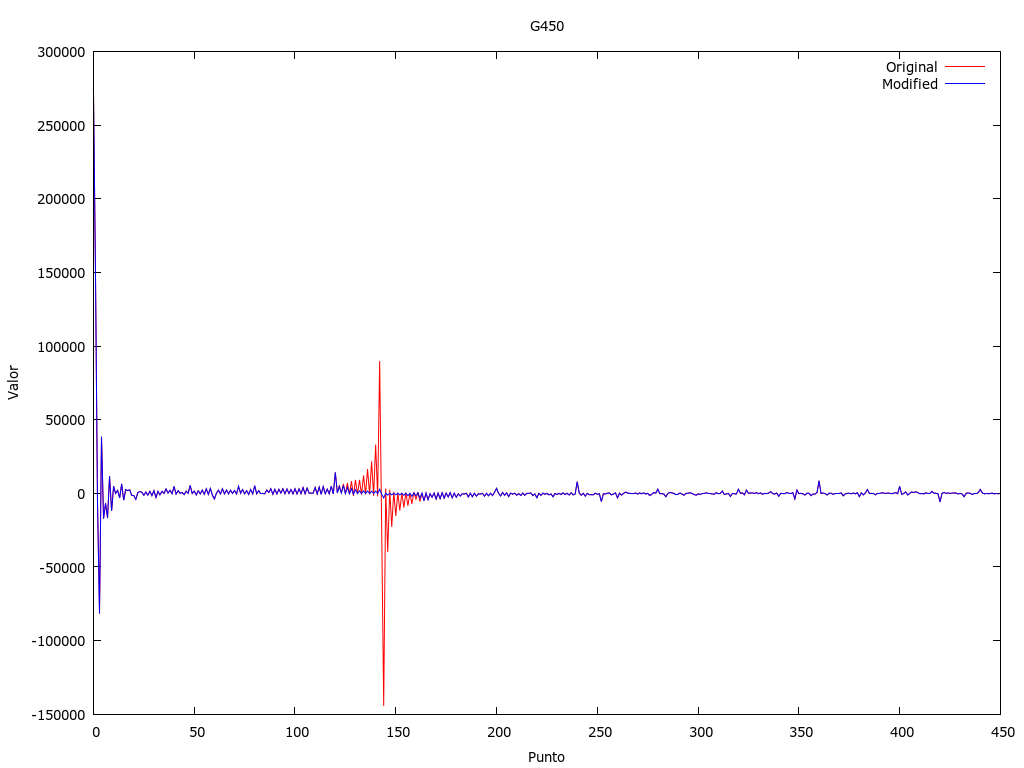
\includegraphics[width=360pt]{imagenes/g450-sin100-exp-spec.png}
\end {center}
\caption{Se\~nal g450 provista por la c\'atedra, transformada, gr\'aficada
luego de aplicar ruido senoidal utilizando el multiplicador 100 (Rojo) y 
habiendo aplicado el filtro exponencial (azul)}
\label{fig:SinProm}
\end{figure}

\begin{figure}
\begin {center}
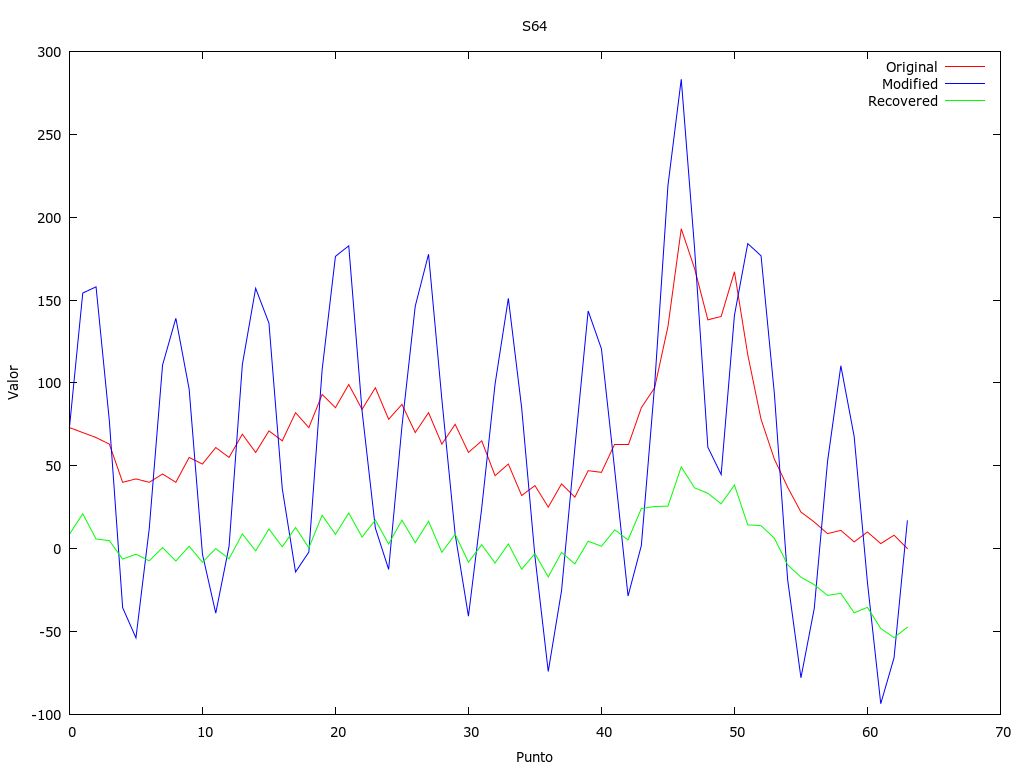
\includegraphics[width=360pt]{imagenes/s64-sin100-exp.png}
\end {center}
\caption{Se\~nal s64 provista por la c\'atedra, no transformada, gr\'aficada
luego de aplicar ruido senoidal utilizando el multiplicador 100 (Rojo) y 
habiendo aplicado el filtro promedio (azul)}
\label{fig:SinProm}
\end{figure}


\subsubsection{Filtro Promedio}

El filtro promedio, en contraposici\'on con el exponencial, toma un promedio
local a la hora de modificar elementos de la se\~nal. Esto se traduce en un
filtro poderoso que devuelve a la se\~nal un estado similar al original.

\begin{figure}
\begin {center}
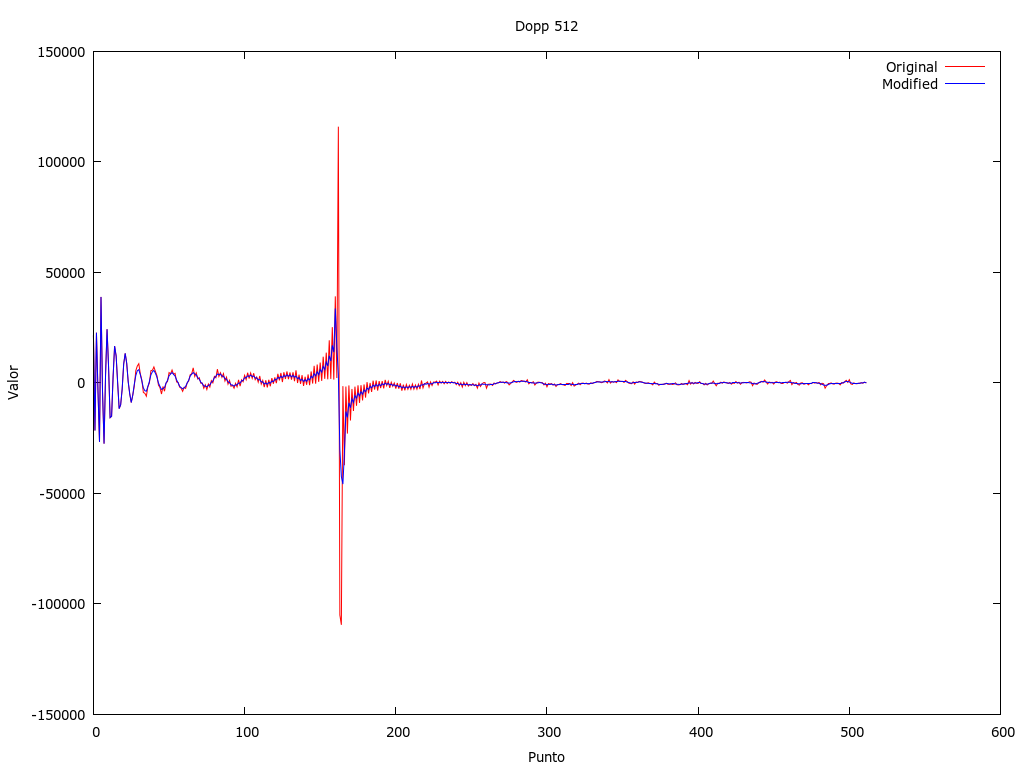
\includegraphics[width=360pt]{imagenes/dopp512-sin100-avg-spec.png}
\end {center}
\caption{Se\~nal doppler provista por la c\'atedra, transformada, gr\'aficada
luego de aplicar ruido senoidal utilizando el multiplicador 100 (Rojo) y 
habiendo aplicado el filtro promedio (azul)}
\label{fig:SinProm}
\end{figure}

\subsubsection{M\'ultiples filtros}

Otra variante utilizada fue la combinaci\'on de los filtros exponencial y
promedio. Al filtrar la se\~nal ruidosa con ambos filtros obtuvimos excelentes
resultados.

\begin{figure}
\begin {center}
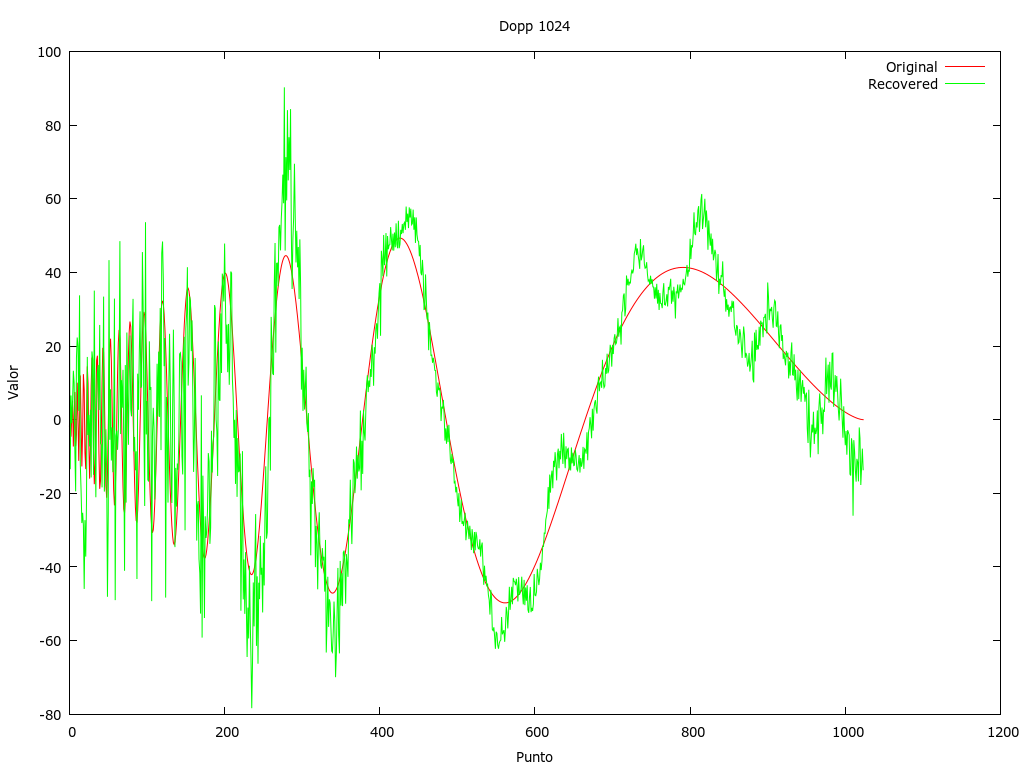
\includegraphics[width=360pt]{imagenes/dopp1024-gauss100-both.png}
\end {center}
\caption{Se\~nal doppler provista por la c\'atedra, no transformada, gr\'aficada
luego de aplicar ruido gaussiano utilizando una amplitud de 100 (Rojo) y 
habiendo aplicado los filtros promedio y exponencial (verde)}
\label{fig:SinProm}
\end{figure}

\begin{figure}
\begin {center}
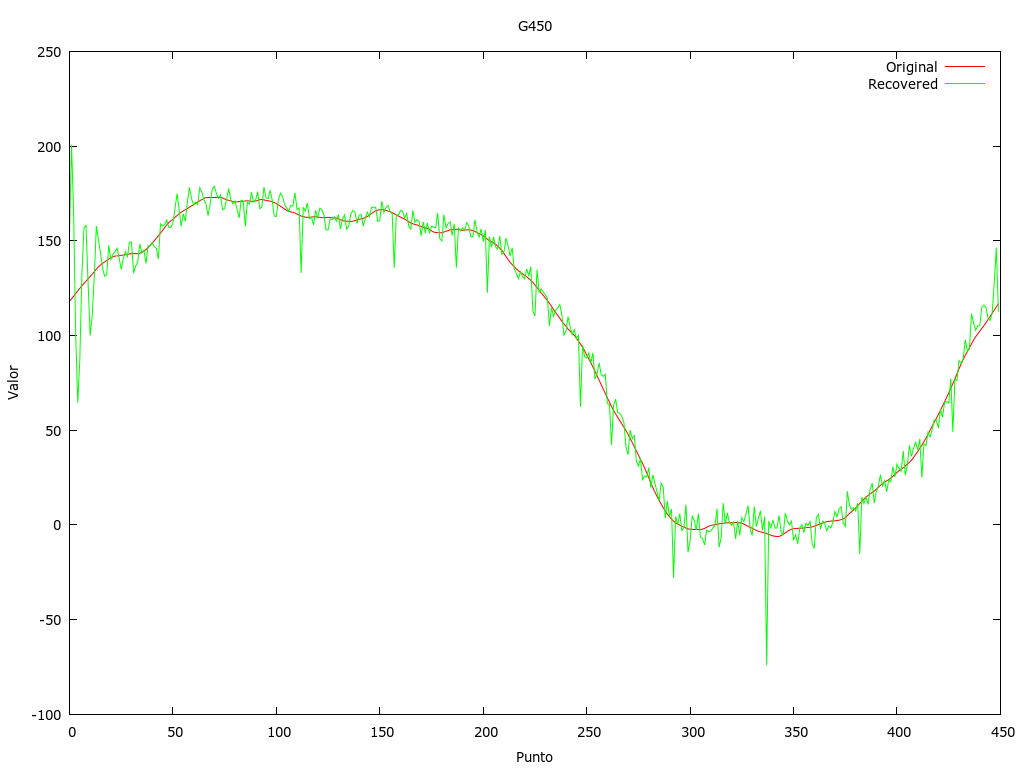
\includegraphics[width=360pt]{imagenes/g450-sin100-both.png}
\end {center}
\caption{Se\~nal g450 provista por la c\'atedra, no transformada, gr\'aficada
luego de aplicar ruido senoidal utilizando el multiplicador 100 (Rojo) y 
habiendo aplicado los filtros promedio y exponencial (verde)}
\label{fig:SinProm}
\end{figure}

\begin{figure}
\begin {center}
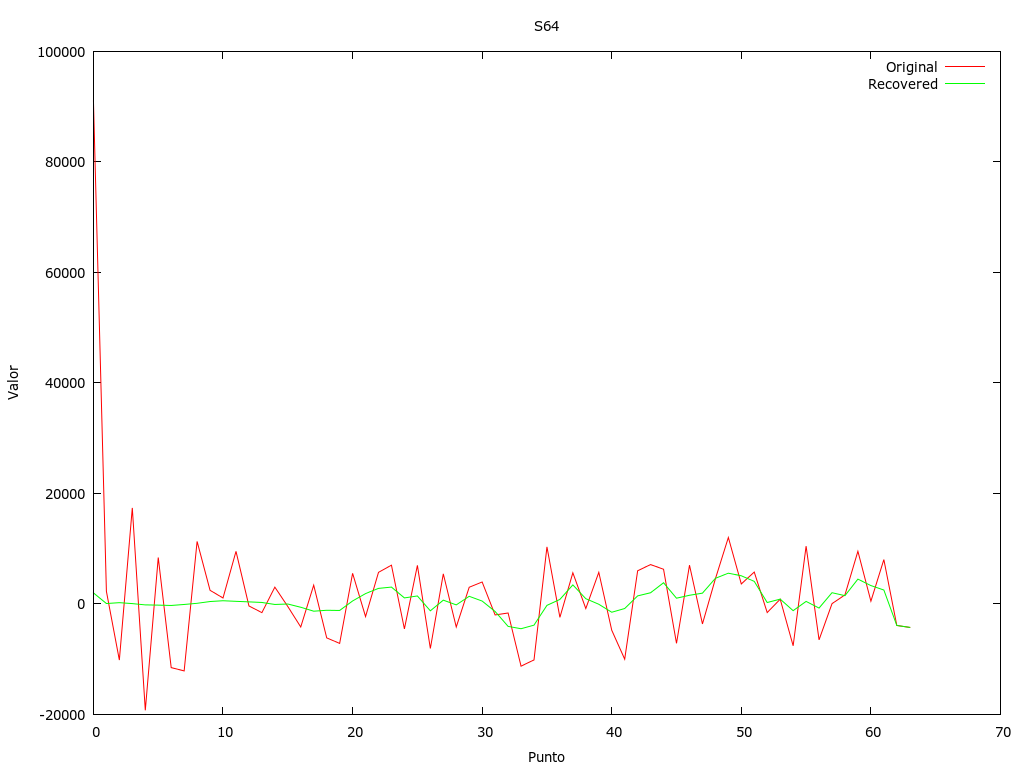
\includegraphics[width=360pt]{imagenes/s64-gauss100-both-spec.png}
\end {center}
\caption{Se\~nal s64 provista por la c\'atedra, transformada, gr\'aficada
luego de aplicar ruido gaussiano utilizando una amplitud de 100 (Rojo) y 
habiendo aplicado los filtros promedio y exponencial (verde)}
\label{fig:SinProm}
\end{figure}


\subsection{Se\~nales en dos dimensiones}

Como fue comentado, durante el desarrollo del experimento se utilizaron
im\'agenes en escala de grises. La imagen tomada como est\'andar y homenaje es 
la de Brian Kernighan.

\begin{figure}[H]
\begin {center}
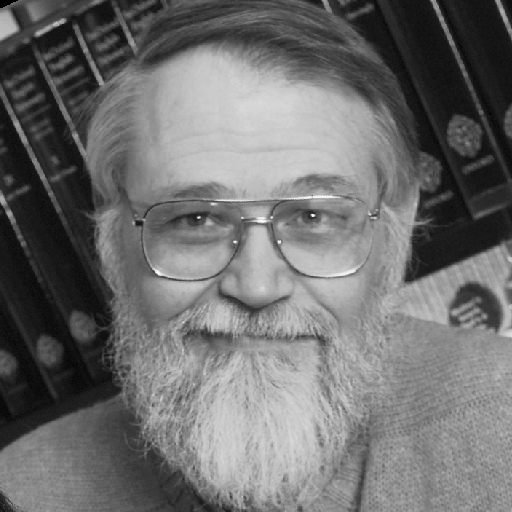
\includegraphics[width=360pt]{imagenes/brian_kernighan.png}
\end {center}
\caption{Imagen original en escala de grises de Brian Kernighan}
\label{fig:SinProm}
\end{figure}

Habiendo mostrado las diferencias entre la implementaci\'on de los filtros en
una dimensi\'on y habiendo portado el filtrado a trav\'es de la toma de cada
fila de la im\'agen como una se\~nal de una dimensi\'on, procedemos a mostrar
los resultados obtenidos en funci\'on de los ruidos aplicados, a diferencia de
lo realizado con una dimensi\'on, donde el foco est\'a puesto en discriminar los
resultados por tipo de filtro.

\subsubsection{Ruido senoidal con multiplicador de 50}

Este ruido es controlado y es as\'i como tambi\'en los filtros pueden volver a
una imagen muy similar a la original.

\begin{figure}[H]
\begin {center}
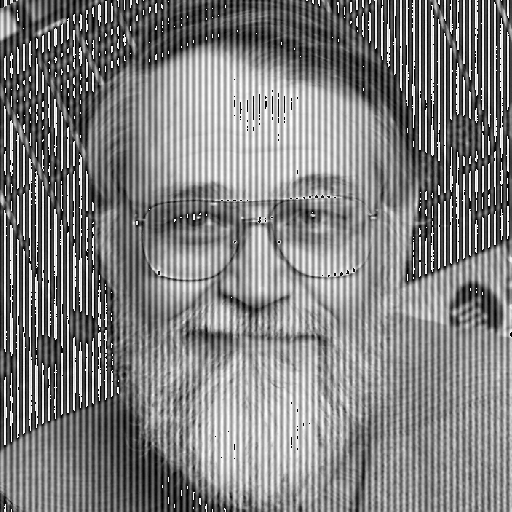
\includegraphics[width=360pt]{imagenes/kern-sin50-noisy.png}
\end {center}
\caption{Imagen con ruido senoidal con multiplicador de 50}
\label{fig:SinProm}
\end{figure}

\begin{figure}[H]
\begin {center}
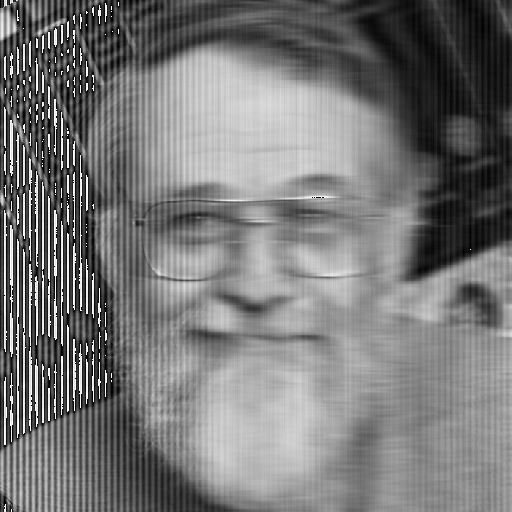
\includegraphics[width=360pt]{imagenes/kern-sin50-recovered-avg.png}
\end {center}
\caption{Recuperada con filtro promedio}
\label{fig:SinProm}
\end{figure}

\begin{figure}[H]
\begin {center}
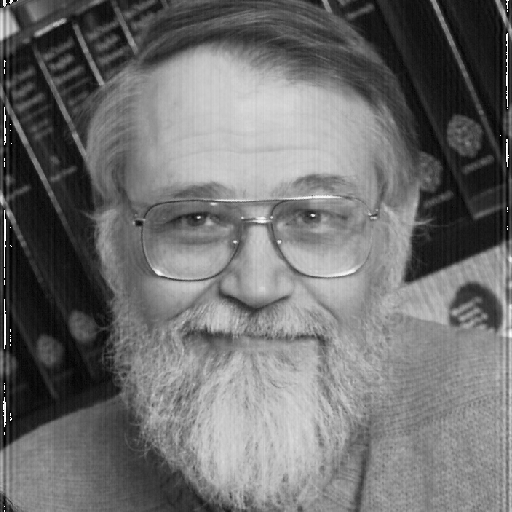
\includegraphics[width=360pt]{imagenes/kern-sin50-recovered.png}
\end {center}
\caption{Recuperada aplicando los 2 filtros}
\label{fig:SinProm}
\end{figure}

\subsubsection{Ruido senoidal con multiplicador de 1000}

Este ruido es controlado pero el multiplicador es muy alto, haciendo muy dificil
la recuperaci\'on de la imagen

\begin{figure}[H]
\begin {center}
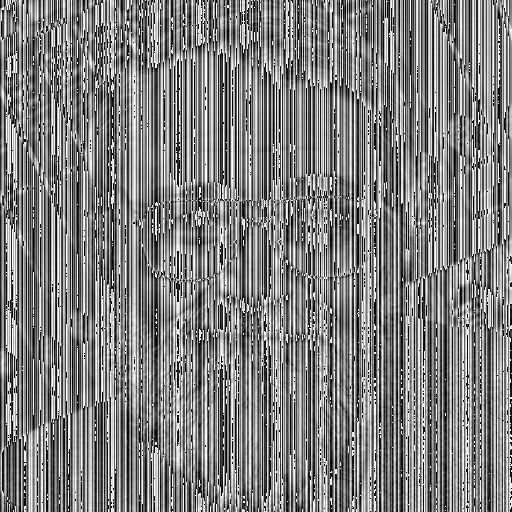
\includegraphics[width=360pt]{imagenes/kern-sin1000-noisy.png}
\end {center}
\caption{Imagen con ruido senoidal con multiplicador de 1000}
\label{fig:SinProm}
\end{figure}

\begin{figure}[H]
\begin {center}
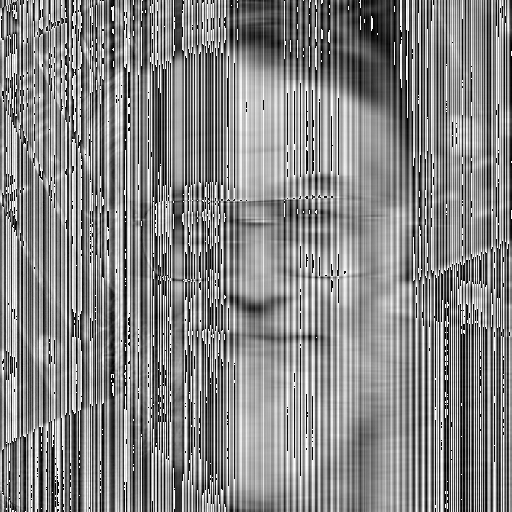
\includegraphics[width=360pt]{imagenes/kern-sin1000-recovered-avg.png}
\end {center}
\caption{Recuperada con filtro promedio}
\label{fig:SinProm}
\end{figure}

\begin{figure}[H]
\begin {center}
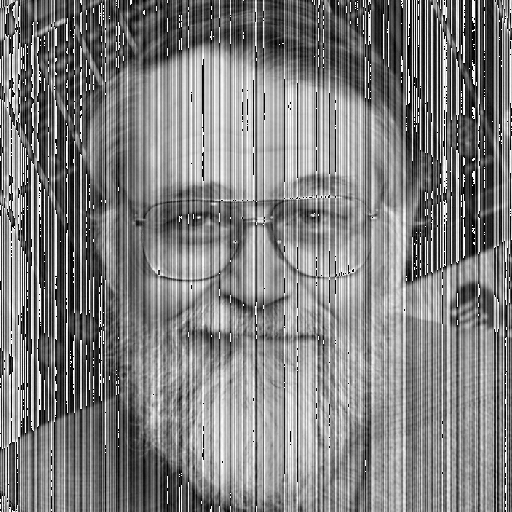
\includegraphics[width=360pt]{imagenes/kern-sin1000-recovered.png}
\end {center}
\caption{Recuperada aplicando los 2 filtros}
\label{fig:SinProm}
\end{figure}


\subsubsection{Ruido gaussiano con factor 100}

Este filtro fue el m\'as desafiante ya que el ruido blanco es muy d\'ificil de
capturar por su condici\'on de ``antipatron''

\begin{figure}[H]
\begin {center}
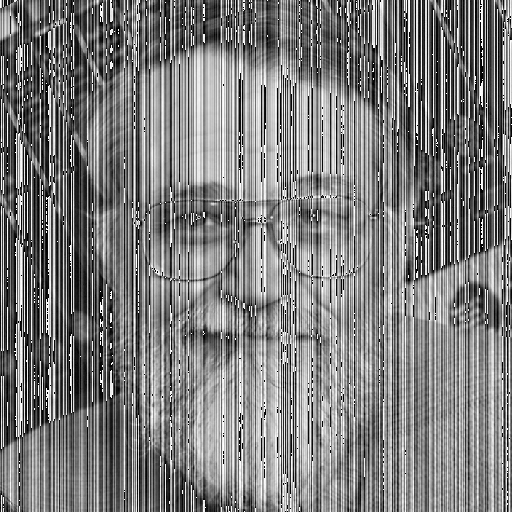
\includegraphics[width=360pt]{imagenes/kern-gauss100-noisy.png}
\end {center}
\caption{Imagen con ruido gaussiano con factor 1000}
\label{fig:SinProm}
\end{figure}

\begin{figure}[H]
\begin {center}
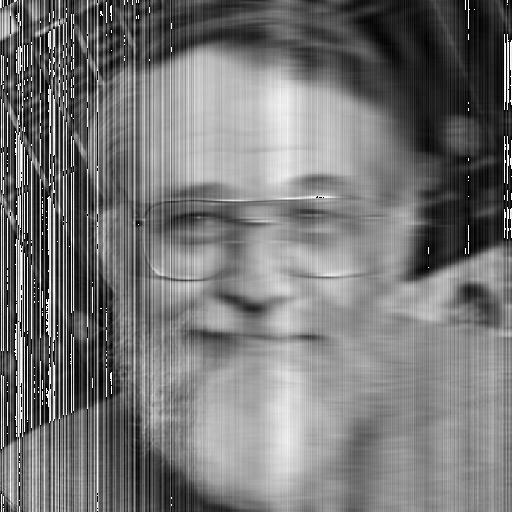
\includegraphics[width=360pt]{imagenes/kern-gauss100-recovered-avg.png}
\end {center}
\caption{Recuperada con filtro promedio}
\label{fig:SinProm}
\end{figure}

\begin{figure}[H]
\begin {center}
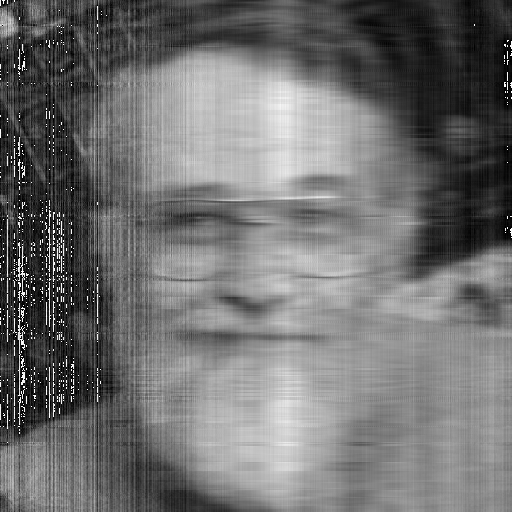
\includegraphics[width=360pt]{imagenes/kern-gauss100-recovered-both.png}
\end {center}
\caption{Recuperada aplicando los 2 filtros}
\label{fig:SinProm}
\end{figure}
